\chapter{Material e método}

\section{Materiais}
\section{Sistema Proposto}
\section{Discussão}

\subsection{Câmera IR}

\todo{Escrever um pouco sobre as câmeras IR}

\section{Construção da câmera IR}

\todo{Um pouco de texto}

\begin{figure}[ht!]
\centering
\fbox{
  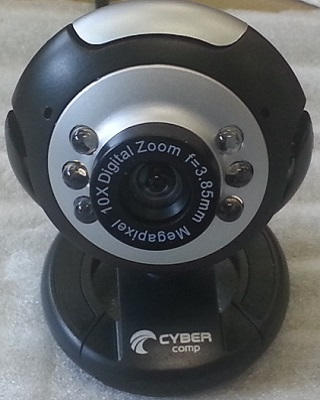
\includegraphics[width=0.3\textwidth]{image/webcam01.jpg}}
  \caption{Webcam sem modificações}
  \label{fig:webcam01}
\end{figure} 

\begin{figure}[ht!]
\centering
\fbox{
  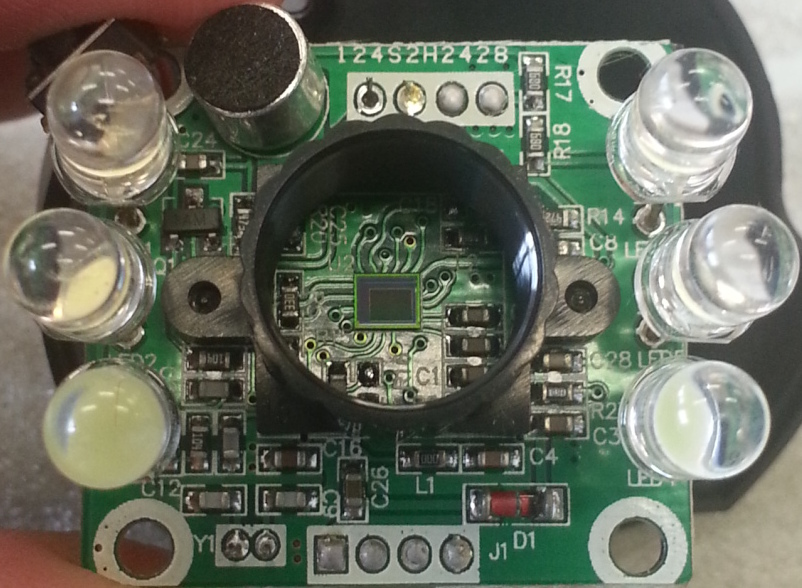
\includegraphics[width=0.3\textwidth]{image/webcam02.jpg}}
  \caption{Webcam sem modificações}
  \label{fig:webcam02}
\end{figure} 

\begin{figure}[ht!]
\centering
\fbox{
  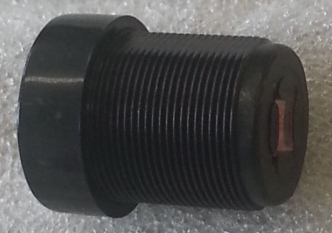
\includegraphics[width=0.3\textwidth]{image/webcam03.jpg}}
  \caption{Webcam sem modificações}
  \label{fig:webcam03}
\end{figure} 

\begin{figure}[ht!]
\centering
\fbox{
  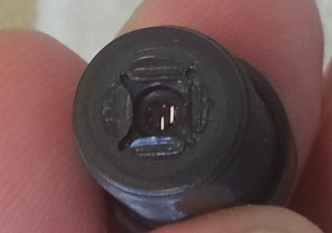
\includegraphics[width=0.3\textwidth]{image/webcam04.jpg}}
  \caption{Webcam sem modificações}
  \label{fig:webcam04}
\end{figure} 

\begin{figure}[ht!]
\centering
\fbox{
  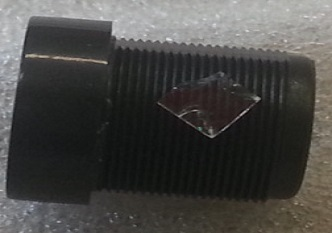
\includegraphics[width=0.3\textwidth]{image/webcam05.jpg}}
  \caption{Webcam sem modificações}
  \label{fig:webcam05}
\end{figure} 

\section{Região de interesse}

Quando o sistema esta inerte e nenhuma mão esta sendo rastreada, podemos criar um região de interesse na imagem para reduzir a área de procura.
